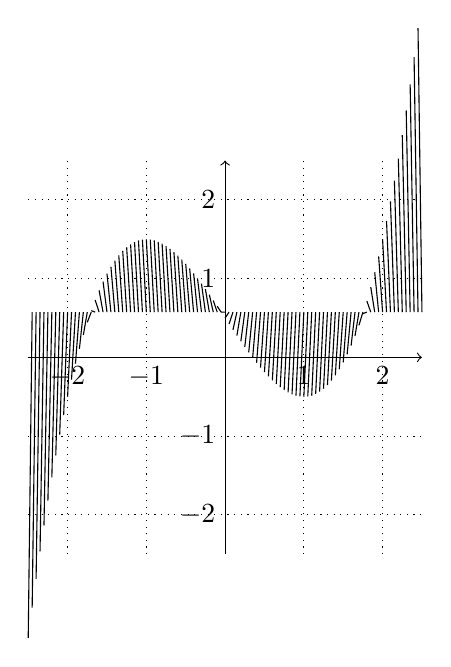
\begin{tikzpicture}
    % Svislá mřížka
    \foreach \x in {-2,...,2} {
        \ifnum \x = 0 {} \else {
            \draw[dotted] (\x, -2.5) -- (\x, 2.5);
            \draw (\x, 0) node[anchor=north] {$\x$};
        } \fi
    }
    % Vodorovná mřížka
    \foreach \y in {-2,...,2} {
        \ifnum \y = 0 {} \else {
            \draw[dotted] (-2.5, \y) -- (2.5, \y);
            \draw (0, \y) node[anchor=east] {$\y$};
        } \fi
    }
    % Osa x a y
    \draw[->] (-2.5, 0) -- (2.5, 0);
    \draw[->] (0, -2.5) -- (0, 2.5);

    % Graf s 100 vzorků
    \foreach \xa in {-2.5, -2.45,...,2.5} {
        \def \xb {\xa + 0.05}
        \def \ya {\xa^3 / 2 - \xa * 3 / 2 + 1 / 2}
        \def \yb {\xb^3 / 2 - \xb * 3 / 2 + 1 / 2}
        \draw (\xa,\ya) -- (\xb,\yb);
    }
\end{tikzpicture}